\documentclass{article}

\usepackage{pdfpages}
\usepackage{graphicx}

\graphicspath{ {./images/} }

\title{
    \vspace{-4.0cm}
    {\Huge Social Routing}\\[0.5cm]    
    \textsc{\Large Project and Seminar}\\[0.5cm]
    \textsc{\large Instituto Superior de Engenharia de Lisboa}\\[0.5cm]
}

\date{\today}
\author{   
    \begin{minipage}{0.4\textwidth}
        \begin{flushleft} \large
        \emph{Authors:}\\
        Baltasar Brito\\
        {\small email: baltasar.brito@gmail.com}\\
        {\small phone: 915953552}\\
        Bernardo Costa\\
        {\small email: bjmcosta97@gmail.com}\\
        {\small phone: 913897555}\\
        \end{flushleft}
    \end{minipage}
    ~
    \begin{minipage}{0.4\textwidth}
        \begin{flushright} \large
        \emph{Supervisor:} \\ 
        Pedro Félix\\
        {\small email: pedrofelix@cc.isel.ipl.pt}\\  
        \end{flushright}
    \end{minipage}\\[2cm]  
}

\begin{document}     
    
    \maketitle
 
    \section{Introduction} 

    %enquadramento,  %descrição clara do projeto,  %citação de literatura já lida;
    %discussão dos problemas a resolver e de possíveis técnicas e ferramentas

        From a tourism perspective, when visiting an unknown place it is usually hard to know which areas to visit without 
        checking either an online or book resource and even then some of the resources might be outdated or business directed 
        (when a restaurant appears in a guide because it payed the guide creators to include it in it for instance). 
        This is what this project aims to solve by providing a quick way to search and undergo user made routes that might include places
        of interest.     

        This solution is materialized in a form of a mobile application and has the following functionalities:
        \begin{itemize}
            \item Route creation.
            \item Ability to search and go on a route, following it in real time on a map.
            \item Route updates and suggestions.
            \item Group messaging through route specific chats, allowing conversations with users in the same route.
        \end{itemize}
    
    %Turn the unknown into a known worth knowing. Explore a new place through a route worth exploring, made by someone
    %who already visited that same place. It's guided exploration.   

    \newpage
    

    \section{Analysis}

        In the context of the application, a route is a path from point A to point B, that goes through user selected sub paths
        that might either have relevance or simply provide the fastest way to the next point of interest of that route. 

        An example of events when using the application might be:

        A user at his hotel decides he wants to go sightseeing for an hour and check the surrounding area by foot.
    
        \begin{itemize}  
            \item The user starts the application and searches for a route inserting his location and time available to spend on a route.
            \item The application suggests the top 3 routes available according to proximity to the user starting point, route evaluation and time necessary to complete the given route. 
            \item The user selects the route and is shown the directions in real time on a map that he has to follow to undergo such route until it is done.
            \item The user finishes the route and evaluates it, with the possibility of adding a suggestion to it. 
        \end{itemize}
        
        \subsection*{Route Creation and Storage}
            The starting point of the application is route creation which has a direct impact on how a route is saved. When in route creation mode, the user
            will be able to see a map where he will be able to add pins to form a route. Each of the pins represents a pair of coordinates and together
            they form the path to follow. Here comes the first problem, should free pin placement be allowed? The solution is a duplicity of input modes, 
            free placement and fixed placement. The first will be used when creating a route in a garden or rural area and the second when in a street (road filled) area. 
            For free placement a line will be drawn directly to the next pin, when on fixed placement the Google Roads API will be used to form a perfect road 
            type path instead of a line that crosses buildings and ignores curves.

        \subsection*{Path to the Route}
            When a route is suggested to a user it must be had in consideration the distance to the starting point of such route, for a route
            is the existing one plus the distance to its beginning. Before suggesting a route to the user this must be taken into consideration,
            specially considering the user's time constraints. There might be a perfect route to such user that is situated 30min away and 
            as such, when suggested, a path to the route must be built and suggested. To be considered also is the case where it's justifiable 
            to include means of transportation to a route, when walking would not be feasible due to the distance and a bus or train would.
        
        \subsection*{Route Ordering}            
            In a scenario where the user is closer to the end than the beginning of a route it 
            might make more sense to start from the end. 
            So an option to consider is to make the route available either in reverse or starting from a specific point of interest.       

        \subsection*{Route Group Chat}
            When a route is started the user is immediately added to that route's chat which gives him the possibility to engage in conversation with other users.
            Of course this is optional and one can chose to do the route alone but this enables another feature when used, the possibility of a guided route,
            or in other words, the pairing of local (regarding the place) users with foreign or unknowledgeable ones.
        
        %todo possible friend system? or too much of a social network resemblance?

    \section{Project Structure}
        The project will be developed in three major components communicating with each other, separating concerns and business logic.
        
        \begin{figure}[h]
            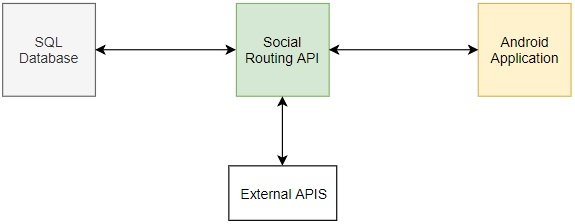
\includegraphics[width=\textwidth]{images/dblocos.png}
        \end{figure} 

        \subsection*{SQL Database}  
            Used to store information regarding each user and created routes. The Social Routing API retrieves user information and is able
            to make better route suggestions to a user because of it. The technologies being considered are MySQL and SQLServer.    

        \subsection*{Social Routing API}
            This http API is responsible for receiving requests from the application component, getting the necessary information from the Database or external APIs
            and responding accordingly. It's in this API that the algorithm for suggesting routes is implemented, the application will only need to show what it
            received from the request.
            Considering the database relational model, the technologies being considered are java and kotlin with usage of the Spring Framework. 
            The external APIs being used are from Google Maps Platform, namely the Google Maps and Google Roads APIs.  

        \subsection*{Android Application}
            In the application resides the visual component of the project, responsible for showing the routes and putting users in contact with each other.
            While it will require internet to be used, the application will have an offline mode, using persistent storage, to check the current route with no internet connection.

    \section{Timeline}   

\end{document}